% Options for packages loaded elsewhere
\PassOptionsToPackage{unicode}{hyperref}
\PassOptionsToPackage{hyphens}{url}
%
\documentclass[
]{article}
\usepackage{amsmath,amssymb}
\usepackage{iftex}
\ifPDFTeX
  \usepackage[T1]{fontenc}
  \usepackage[utf8]{inputenc}
  \usepackage{textcomp} % provide euro and other symbols
\else % if luatex or xetex
  \usepackage{unicode-math} % this also loads fontspec
  \defaultfontfeatures{Scale=MatchLowercase}
  \defaultfontfeatures[\rmfamily]{Ligatures=TeX,Scale=1}
\fi
\usepackage{lmodern}
\ifPDFTeX\else
  % xetex/luatex font selection
\fi
% Use upquote if available, for straight quotes in verbatim environments
\IfFileExists{upquote.sty}{\usepackage{upquote}}{}
\IfFileExists{microtype.sty}{% use microtype if available
  \usepackage[]{microtype}
  \UseMicrotypeSet[protrusion]{basicmath} % disable protrusion for tt fonts
}{}
\makeatletter
\@ifundefined{KOMAClassName}{% if non-KOMA class
  \IfFileExists{parskip.sty}{%
    \usepackage{parskip}
  }{% else
    \setlength{\parindent}{0pt}
    \setlength{\parskip}{6pt plus 2pt minus 1pt}}
}{% if KOMA class
  \KOMAoptions{parskip=half}}
\makeatother
\usepackage{xcolor}
\usepackage[margin=1in]{geometry}
\usepackage{color}
\usepackage{fancyvrb}
\newcommand{\VerbBar}{|}
\newcommand{\VERB}{\Verb[commandchars=\\\{\}]}
\DefineVerbatimEnvironment{Highlighting}{Verbatim}{commandchars=\\\{\}}
% Add ',fontsize=\small' for more characters per line
\usepackage{framed}
\definecolor{shadecolor}{RGB}{248,248,248}
\newenvironment{Shaded}{\begin{snugshade}}{\end{snugshade}}
\newcommand{\AlertTok}[1]{\textcolor[rgb]{0.94,0.16,0.16}{#1}}
\newcommand{\AnnotationTok}[1]{\textcolor[rgb]{0.56,0.35,0.01}{\textbf{\textit{#1}}}}
\newcommand{\AttributeTok}[1]{\textcolor[rgb]{0.13,0.29,0.53}{#1}}
\newcommand{\BaseNTok}[1]{\textcolor[rgb]{0.00,0.00,0.81}{#1}}
\newcommand{\BuiltInTok}[1]{#1}
\newcommand{\CharTok}[1]{\textcolor[rgb]{0.31,0.60,0.02}{#1}}
\newcommand{\CommentTok}[1]{\textcolor[rgb]{0.56,0.35,0.01}{\textit{#1}}}
\newcommand{\CommentVarTok}[1]{\textcolor[rgb]{0.56,0.35,0.01}{\textbf{\textit{#1}}}}
\newcommand{\ConstantTok}[1]{\textcolor[rgb]{0.56,0.35,0.01}{#1}}
\newcommand{\ControlFlowTok}[1]{\textcolor[rgb]{0.13,0.29,0.53}{\textbf{#1}}}
\newcommand{\DataTypeTok}[1]{\textcolor[rgb]{0.13,0.29,0.53}{#1}}
\newcommand{\DecValTok}[1]{\textcolor[rgb]{0.00,0.00,0.81}{#1}}
\newcommand{\DocumentationTok}[1]{\textcolor[rgb]{0.56,0.35,0.01}{\textbf{\textit{#1}}}}
\newcommand{\ErrorTok}[1]{\textcolor[rgb]{0.64,0.00,0.00}{\textbf{#1}}}
\newcommand{\ExtensionTok}[1]{#1}
\newcommand{\FloatTok}[1]{\textcolor[rgb]{0.00,0.00,0.81}{#1}}
\newcommand{\FunctionTok}[1]{\textcolor[rgb]{0.13,0.29,0.53}{\textbf{#1}}}
\newcommand{\ImportTok}[1]{#1}
\newcommand{\InformationTok}[1]{\textcolor[rgb]{0.56,0.35,0.01}{\textbf{\textit{#1}}}}
\newcommand{\KeywordTok}[1]{\textcolor[rgb]{0.13,0.29,0.53}{\textbf{#1}}}
\newcommand{\NormalTok}[1]{#1}
\newcommand{\OperatorTok}[1]{\textcolor[rgb]{0.81,0.36,0.00}{\textbf{#1}}}
\newcommand{\OtherTok}[1]{\textcolor[rgb]{0.56,0.35,0.01}{#1}}
\newcommand{\PreprocessorTok}[1]{\textcolor[rgb]{0.56,0.35,0.01}{\textit{#1}}}
\newcommand{\RegionMarkerTok}[1]{#1}
\newcommand{\SpecialCharTok}[1]{\textcolor[rgb]{0.81,0.36,0.00}{\textbf{#1}}}
\newcommand{\SpecialStringTok}[1]{\textcolor[rgb]{0.31,0.60,0.02}{#1}}
\newcommand{\StringTok}[1]{\textcolor[rgb]{0.31,0.60,0.02}{#1}}
\newcommand{\VariableTok}[1]{\textcolor[rgb]{0.00,0.00,0.00}{#1}}
\newcommand{\VerbatimStringTok}[1]{\textcolor[rgb]{0.31,0.60,0.02}{#1}}
\newcommand{\WarningTok}[1]{\textcolor[rgb]{0.56,0.35,0.01}{\textbf{\textit{#1}}}}
\usepackage{graphicx}
\makeatletter
\def\maxwidth{\ifdim\Gin@nat@width>\linewidth\linewidth\else\Gin@nat@width\fi}
\def\maxheight{\ifdim\Gin@nat@height>\textheight\textheight\else\Gin@nat@height\fi}
\makeatother
% Scale images if necessary, so that they will not overflow the page
% margins by default, and it is still possible to overwrite the defaults
% using explicit options in \includegraphics[width, height, ...]{}
\setkeys{Gin}{width=\maxwidth,height=\maxheight,keepaspectratio}
% Set default figure placement to htbp
\makeatletter
\def\fps@figure{htbp}
\makeatother
\setlength{\emergencystretch}{3em} % prevent overfull lines
\providecommand{\tightlist}{%
  \setlength{\itemsep}{0pt}\setlength{\parskip}{0pt}}
\setcounter{secnumdepth}{-\maxdimen} % remove section numbering
\usepackage{tcolorbox}
\usepackage{etoolbox}
\usepackage{framed}

\tcbuselibrary{skins} % Habilita recursos extras do tcolorbox

% Configuração para blocos de código (verbatim)
\BeforeBeginEnvironment{verbatim}{%
	\begin{tcolorbox}[colback=gray!5!white, colframe=gray!80!black, arc=3pt, boxrule=0.1pt]%
	}
	\AfterEndEnvironment{verbatim}{%
	\end{tcolorbox}%
}
\setcounter{page}{2}
\usepackage{fvextra}
\usepackage{tcolorbox}
\tcbuselibrary{breakable}
\usepackage{xcolor}
\DefineVerbatimEnvironment{verbatim}{Verbatim}{
  breaklines=true,
  breakanywhere=true,
  fontsize=\small}

\usepackage{float}
\ifLuaTeX
  \usepackage{selnolig}  % disable illegal ligatures
\fi
\usepackage{bookmark}
\IfFileExists{xurl.sty}{\usepackage{xurl}}{} % add URL line breaks if available
\urlstyle{same}
\hypersetup{
  hidelinks,
  pdfcreator={LaTeX via pandoc}}

\author{}
\date{\vspace{-2.5em}}

\begin{document}

\begin{center}
    {\LARGE \bfseries Projeto em grupo - Versão 2}
    
\end{center}

\subsection{Informações iniciais}\label{informauxe7uxf5es-iniciais}

\begin{itemize}
\item
  \textbf{Título do artigo:} \emph{``Optimizing self-organized study
  orders: combining refutations and metacognitive prompts improves the
  use of interleaved practice''}
\item
  \textbf{Link do artigo:}
  \textcolor{blue}{\underline{\url{https://www.nature.com/articles/s41539-024-00245-7\#Sec9}}}
\item
  \textbf{Dados:}
  \textcolor{blue}{\underline{\url{https://osf.io/6vm7z/?view_only=d9caf564f48b4c4f8166b3c2e38c1cf4}}}
\item
  \textbf{Dicionário dos dados:}
  \textcolor{blue}{\underline{\url{https://dataverse.nl/dataset.xhtml?persistentId=doi:10.34894/U9YSER}}}
\end{itemize}

\subsection{Contextualização}\label{contextualizauxe7uxe3o}

O artigo discute sobre a organização de estudos durante a aprendizagem
por categorias e suas práticas: a prática intercalada (\emph{interleaved
practice}), que consiste na alternância de estudo entre diferentes
categorias/conceitos, e a prática por blocos (\emph{blocked practice}),
que consiste no estudo de uma categoria/conceito por vez.

A prática de estudo por blocos costuma ser frequentemente escolhida
pelos estudantes, em detrimento da prática intercalada, mas pesquisas
recentes passaram a informar que a prática intercalada é uma estratégia
mais efetiva. Nesse contexto, diversos estudos são realizados a partir
de testes com estudantes, testes esses que predefinem uma ordem de
estudos. Mas nunca houve um teste que fosse realizado de forma que os
próprios estudantes definissem uma ordem de estudos para eles mesmos.

Nesse sentido, foi realizado neste artigo um experimento com 91
estudantes universitários, que consistiu nas seguintes etapas:

\begin{itemize}
\item
  Divisão dos estudantes em grupos controle e teste;
\item
  Exposição dos estudantes do grupo de teste a intervenções: que
  consistiram na leitura de textos e avisos metacognitivos que destacam
  a superioridade da prática intercalada de estudos em detrimento à
  prática por blocos, ou seja, refutações do que comumente acreditam.
\end{itemize}

\subsection{Análises realizadas/resultados
obtidos}\label{anuxe1lises-realizadasresultados-obtidos}

Para analisar os dados obtidos na pesquisa, foram elaboradas três RQs
(\emph{good research questions}):

\subsubsection{\texorpdfstring{\emph{RQ1. Learning strategy beliefs
across time and between
conditions}}{RQ1. Learning strategy beliefs across time and between conditions}}\label{rq1.-learning-strategy-beliefs-across-time-and-between-conditions}

\begin{quote}
Como a crença dos participantes nas diferentes estratégias de
aprendizado (em blocos/intercalada) variou com o tempo e entre as
condições?
\end{quote}

Esta RQ avaliou a influência da intervenção das crenças nas estratégias
de aprendizagem (intercalada e por blocos). Para isso, foram aplicados
três testes estatísticos:

\begin{itemize}
\item
  \textbf{Teste t para amostras pareadas}: para analisar a crença pré
  existente dos participantes;
\item
  \textbf{ANOVA mista}: para observar a variância ao longo do tempo,
  separando por grupo intervenção e grupo controle;
\item
  \textbf{Comparação pareada com Bonferroni}.
\end{itemize}

Para responder à cada uma das RQs, primeiro faremos um \emph{setup}
inicial (importação de bibliotecas necessárias e leitura dos dadoss).

\begin{Shaded}
\begin{Highlighting}[]
\CommentTok{\# Importação de bibliotecas}
\FunctionTok{library}\NormalTok{(afex)}
\FunctionTok{library}\NormalTok{(emmeans)}

\CommentTok{\# Leitura dos dados}
\NormalTok{url\_csv }\OtherTok{=} \FunctionTok{paste0}\NormalTok{(}
  \StringTok{"https://docs.google.com/spreadsheets/d/"}\NormalTok{,}
  \StringTok{"1Fv6oRXMtoDKcbS19awogukMpTLr5utXLJ3aw8GXzGbA/"}\NormalTok{,}
  \StringTok{"export?format=csv\&gid=2113233241"}\NormalTok{)}

\NormalTok{dados }\OtherTok{=} \FunctionTok{read.csv}\NormalTok{(}\AttributeTok{file =}\NormalTok{ url\_csv, }\AttributeTok{sep=}\StringTok{","}\NormalTok{, }\AttributeTok{header=}\ConstantTok{TRUE}\NormalTok{)}
\end{Highlighting}
\end{Shaded}

Agora, seguindo para a aplicação dos testes:

\textbf{1.1 - Teste t para amostras pareadas}

\begin{Shaded}
\begin{Highlighting}[]
\CommentTok{\# RQ1 {-} Crenças pré existentes}

\CommentTok{\# Percepção efetiva *blocked practice*}
\NormalTok{PE\_B1 }\OtherTok{=}\NormalTok{ dados}\SpecialCharTok{$}\NormalTok{PE\_B1}

\CommentTok{\# Média e desvio padrão}
\FunctionTok{c}\NormalTok{(}\FunctionTok{floor}\NormalTok{(}\FunctionTok{mean}\NormalTok{(PE\_B1)}\SpecialCharTok{*}\DecValTok{100}\NormalTok{)}\SpecialCharTok{/}\DecValTok{100}\NormalTok{, }\FunctionTok{round}\NormalTok{(}\FunctionTok{sd}\NormalTok{(PE\_B1), }\DecValTok{2}\NormalTok{))}
\end{Highlighting}
\end{Shaded}

\begin{verbatim}
## [1] 4.39 0.85
\end{verbatim}

\begin{Shaded}
\begin{Highlighting}[]
\CommentTok{\# A amostra não passou no teste de normalidade}
\FunctionTok{shapiro.test}\NormalTok{(PE\_B1)}
\end{Highlighting}
\end{Shaded}

\begin{verbatim}
## 
##  Shapiro-Wilk normality test
## 
## data:  PE_B1
## W = 0.86596, p-value = 1.433e-07
\end{verbatim}

\begin{Shaded}
\begin{Highlighting}[]
\CommentTok{\# Observando a distribuição}
\FunctionTok{hist}\NormalTok{(PE\_B1, }\AttributeTok{prob=}\ConstantTok{TRUE}\NormalTok{)}
\end{Highlighting}
\end{Shaded}

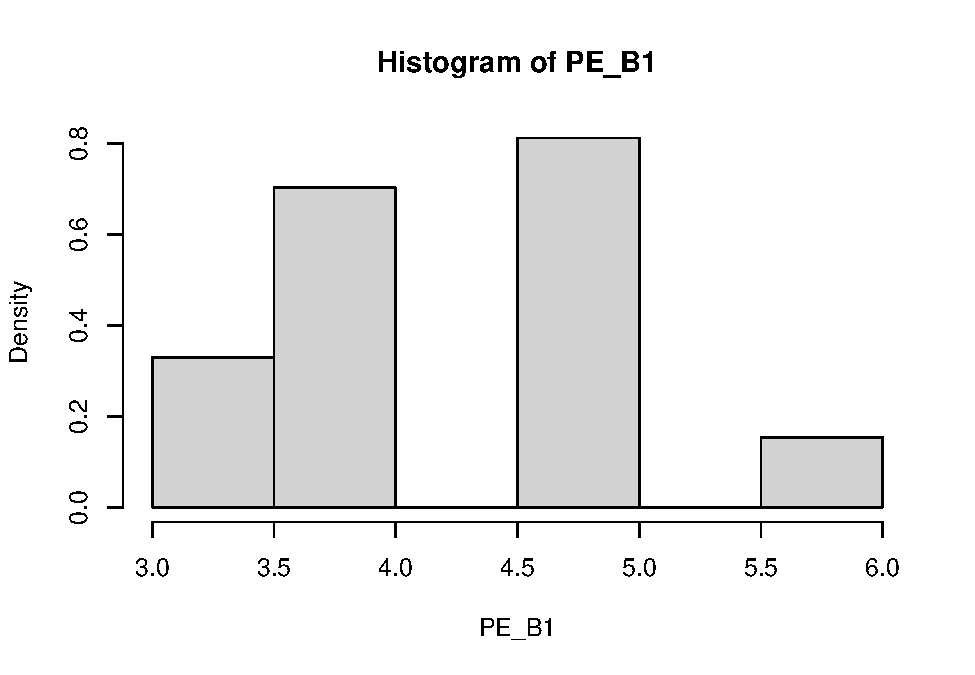
\includegraphics{Projeto_em_grupo_versao-2--pdf-_files/figure-latex/unnamed-chunk-2-1.pdf}

\begin{Shaded}
\begin{Highlighting}[]
\CommentTok{\# Percepção efetiva *interleaved practice*}
\NormalTok{PE\_I1 }\OtherTok{=}\NormalTok{ dados}\SpecialCharTok{$}\NormalTok{PE\_I1}

\CommentTok{\# Média e desvio padrão}
\FunctionTok{c}\NormalTok{(}\FunctionTok{round}\NormalTok{(}\FunctionTok{mean}\NormalTok{(PE\_I1), }\DecValTok{3}\NormalTok{), }\FunctionTok{round}\NormalTok{(}\FunctionTok{sd}\NormalTok{(PE\_I1), }\DecValTok{2}\NormalTok{))}
\end{Highlighting}
\end{Shaded}

\begin{verbatim}
## [1] 4.00 1.02
\end{verbatim}

\begin{Shaded}
\begin{Highlighting}[]
\CommentTok{\# A amostra não passou no teste de normalidade}
\FunctionTok{shapiro.test}\NormalTok{(PE\_I1)}
\end{Highlighting}
\end{Shaded}

\begin{verbatim}
## 
##  Shapiro-Wilk normality test
## 
## data:  PE_I1
## W = 0.88318, p-value = 6.869e-07
\end{verbatim}

\begin{Shaded}
\begin{Highlighting}[]
\CommentTok{\# Observando a distribuição}
\FunctionTok{hist}\NormalTok{(PE\_I1, }\AttributeTok{prob=}\ConstantTok{TRUE}\NormalTok{)}
\end{Highlighting}
\end{Shaded}

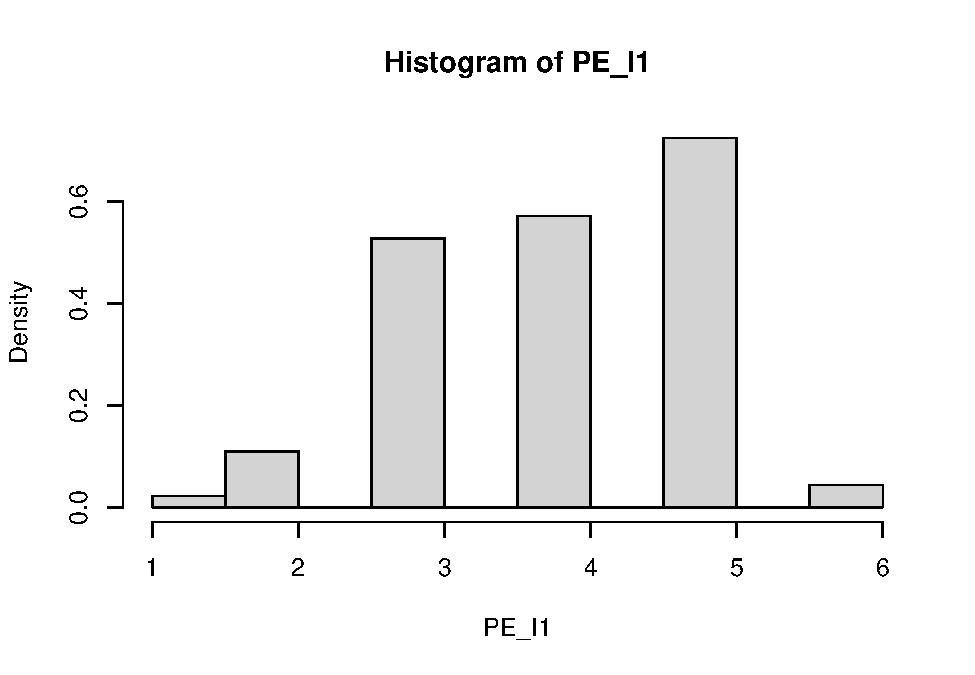
\includegraphics{Projeto_em_grupo_versao-2--pdf-_files/figure-latex/unnamed-chunk-2-2.pdf}

\begin{Shaded}
\begin{Highlighting}[]
\CommentTok{\# teste t pareado}

\CommentTok{\# H0: mu(PE\_B1) = mu(PE\_I1)}
\CommentTok{\# Ha: mu(PE\_B1) != mu(PE\_I1)}
\FunctionTok{t.test}\NormalTok{(PE\_B1, PE\_I1, }\AttributeTok{mu=}\DecValTok{0}\NormalTok{, }\AttributeTok{paired=}\ConstantTok{TRUE}\NormalTok{)}
\end{Highlighting}
\end{Shaded}

\begin{verbatim}
## 
##  Paired t-test
## 
## data:  PE_B1 and PE_I1
## t = 2.3619, df = 90, p-value = 0.02034
## alternative hypothesis: true mean difference is not equal to 0
## 95 percent confidence interval:
##  0.06285266 0.72835613
## sample estimates:
## mean difference 
##       0.3956044
\end{verbatim}

Pelos resultados do \emph{teste t}, a hipótese nula é rejeitada, devido
à obtenção de um \textbf{p-valor} (\(0.020\)) menor que
\(\alpha = 0.05\).

\textbf{1.2 - ANOVA: variância ao longo do tempo - usando o pacote
\texttt{afex}}

Como a crença nas diferentes técnicas de estudo variou com o
tempo/condição?

\textbf{Setup}

\begin{Shaded}
\begin{Highlighting}[]
\CommentTok{\# Transformação de dados}
\NormalTok{dados\_limpos }\OtherTok{=} \FunctionTok{na.omit}\NormalTok{(dados)}

\NormalTok{dados\_ANOVA\_RQ1 }\OtherTok{=} \FunctionTok{data.frame}\NormalTok{(}
    \FunctionTok{rep}\NormalTok{(dados\_limpos}\SpecialCharTok{$}\NormalTok{DM08\_01, }\DecValTok{3}\NormalTok{),}
    \FunctionTok{c}\NormalTok{(}\FunctionTok{rep}\NormalTok{(}\StringTok{\textquotesingle{}pre{-}intervention\textquotesingle{}}\NormalTok{, }\DecValTok{89}\NormalTok{),}
      \FunctionTok{rep}\NormalTok{(}\StringTok{\textquotesingle{}post{-}intervention\textquotesingle{}}\NormalTok{, }\DecValTok{89}\NormalTok{), }\FunctionTok{rep}\NormalTok{(}\StringTok{\textquotesingle{}after a delay\textquotesingle{}}\NormalTok{, }\DecValTok{89}\NormalTok{)),}
    \FunctionTok{c}\NormalTok{(dados\_limpos}\SpecialCharTok{$}\NormalTok{PE\_B1, dados\_limpos}\SpecialCharTok{$}\NormalTok{PE\_B2, dados\_limpos}\SpecialCharTok{$}\NormalTok{PE\_B3),}
    \FunctionTok{c}\NormalTok{(dados\_limpos}\SpecialCharTok{$}\NormalTok{PE\_I1, dados\_limpos}\SpecialCharTok{$}\NormalTok{PE\_I2, dados\_limpos}\SpecialCharTok{$}\NormalTok{PE\_I3),}
    \FunctionTok{rep}\NormalTok{(dados\_limpos}\SpecialCharTok{$}\NormalTok{Condition, }\DecValTok{3}\NormalTok{)}
\NormalTok{)}
\FunctionTok{colnames}\NormalTok{(dados\_ANOVA\_RQ1) }\OtherTok{\textless{}{-}} \FunctionTok{c}\NormalTok{(}\StringTok{"id"}\NormalTok{, }\StringTok{"tempo"}\NormalTok{, }\StringTok{"percep\_blocked"}\NormalTok{,}
                               \StringTok{"percep\_interleaved"}\NormalTok{, }\StringTok{"condicao"}\NormalTok{)}

\NormalTok{dados\_ANOVA\_RQ1\_filtro\_grupo\_intervencao }\OtherTok{=}\NormalTok{ (}
\NormalTok{  dados\_ANOVA\_RQ1[dados\_ANOVA\_RQ1}\SpecialCharTok{$}\NormalTok{condicao }\SpecialCharTok{==} \StringTok{"Full"}\NormalTok{, ])}

\NormalTok{dados\_ANOVA\_RQ1\_filtro\_grupo\_controle }\OtherTok{=}\NormalTok{ (}
\NormalTok{  dados\_ANOVA\_RQ1[dados\_ANOVA\_RQ1}\SpecialCharTok{$}\NormalTok{condicao }\SpecialCharTok{==} \StringTok{"Control"}\NormalTok{, ])}

\CommentTok{\# Visualização das 15 primeiras linhas dataframe transformado}

\FunctionTok{head}\NormalTok{(dados\_ANOVA\_RQ1, }\DecValTok{15}\NormalTok{)}
\end{Highlighting}
\end{Shaded}

\begin{verbatim}
##    id            tempo percep_blocked percep_interleaved condicao
## 1   1 pre-intervention              5                  3  Control
## 2   2 pre-intervention              6                  4  Control
## 3   3 pre-intervention              4                  5  Control
## 4   4 pre-intervention              4                  3  Control
## 5   5 pre-intervention              4                  3  Control
## 6   6 pre-intervention              5                  4     Full
## 7   7 pre-intervention              4                  4  Control
## 8   8 pre-intervention              5                  4     Full
## 9   9 pre-intervention              5                  4     Full
## 10 10 pre-intervention              5                  3     Full
## 11 11 pre-intervention              5                  3     Full
## 12 12 pre-intervention              5                  4  Control
## 13 13 pre-intervention              4                  5  Control
## 14 14 pre-intervention              4                  5  Control
## 15 15 pre-intervention              3                  5  Control
\end{verbatim}

\textbf{1.2.1 - Criação dos modelos ANOVA}

\begin{Shaded}
\begin{Highlighting}[]
\CommentTok{\# Modelos ANOVA {-}{-} os valores nulos foram desconsiderados}

\CommentTok{\# Variáveis preditoras}
\CommentTok{\# tempo ; condicao}

\CommentTok{\# Variáveis resposta}
\CommentTok{\# percep\_blocked; percep\_interleaved}

\CommentTok{\# Função para rodar ANOVA mista}
\NormalTok{rodar\_anova }\OtherTok{\textless{}{-}} \ControlFlowTok{function}\NormalTok{(dv, dados, }\AttributeTok{between =} \ConstantTok{TRUE}\NormalTok{) \{}
  \ControlFlowTok{if}\NormalTok{ (between) \{}
    \FunctionTok{aov\_ez}\NormalTok{(}\AttributeTok{id =} \StringTok{"id"}\NormalTok{, }\AttributeTok{dv =}\NormalTok{ dv, }\AttributeTok{data =}\NormalTok{ dados, }\AttributeTok{within =} \StringTok{"tempo"}\NormalTok{,}
           \AttributeTok{between =} \StringTok{"condicao"}\NormalTok{)}
\NormalTok{  \} }\ControlFlowTok{else}\NormalTok{ \{}
    \FunctionTok{aov\_ez}\NormalTok{(}\AttributeTok{id =} \StringTok{"id"}\NormalTok{, }\AttributeTok{dv =}\NormalTok{ dv, }\AttributeTok{data =}\NormalTok{ dados, }\AttributeTok{within =} \StringTok{"tempo"}\NormalTok{)}
\NormalTok{  \}}
\NormalTok{\}}

\CommentTok{\# Modelos gerais (com fator entre{-}sujeitos)}
\NormalTok{modelo\_blocked }\OtherTok{\textless{}{-}} \FunctionTok{rodar\_anova}\NormalTok{(}\StringTok{"percep\_blocked"}\NormalTok{, dados\_ANOVA\_RQ1)}
\end{Highlighting}
\end{Shaded}

\begin{verbatim}
## Converting to factor: condicao
\end{verbatim}

\begin{verbatim}
## Contrasts set to contr.sum for the following variables: condicao
\end{verbatim}

\begin{Shaded}
\begin{Highlighting}[]
\NormalTok{modelo\_interleaved }\OtherTok{\textless{}{-}} \FunctionTok{rodar\_anova}\NormalTok{(}\StringTok{"percep\_interleaved"}\NormalTok{, dados\_ANOVA\_RQ1)}
\end{Highlighting}
\end{Shaded}

\begin{verbatim}
## Converting to factor: condicao
## Contrasts set to contr.sum for the following variables: condicao
\end{verbatim}

\begin{Shaded}
\begin{Highlighting}[]
\CommentTok{\# Modelos separados por grupo (sem fator entre{-}sujeitos)}
\NormalTok{modelo\_blocked\_interv }\OtherTok{\textless{}{-}} \FunctionTok{rodar\_anova}\NormalTok{(}\StringTok{"percep\_blocked"}\NormalTok{,}
\NormalTok{                                     dados\_ANOVA\_RQ1\_filtro\_grupo\_intervencao,}
                                     \AttributeTok{between =} \ConstantTok{FALSE}\NormalTok{)}

\NormalTok{modelo\_blocked\_control }\OtherTok{\textless{}{-}} \FunctionTok{rodar\_anova}\NormalTok{(}\StringTok{"percep\_blocked"}\NormalTok{,}
\NormalTok{                                      dados\_ANOVA\_RQ1\_filtro\_grupo\_controle,}
                                      \AttributeTok{between =} \ConstantTok{FALSE}\NormalTok{)}

\NormalTok{modelo\_interleaved\_interv }\OtherTok{\textless{}{-}} \FunctionTok{rodar\_anova}\NormalTok{(}
  \StringTok{"percep\_interleaved"}\NormalTok{,}
\NormalTok{  dados\_ANOVA\_RQ1\_filtro\_grupo\_intervencao,}
  \AttributeTok{between =} \ConstantTok{FALSE}\NormalTok{)}

\NormalTok{modelo\_interleaved\_control }\OtherTok{\textless{}{-}} \FunctionTok{rodar\_anova}\NormalTok{(}
  \StringTok{"percep\_interleaved"}\NormalTok{,}
\NormalTok{  dados\_ANOVA\_RQ1\_filtro\_grupo\_controle,}
  \AttributeTok{between =} \ConstantTok{FALSE}\NormalTok{)}
\end{Highlighting}
\end{Shaded}

\textbf{1.2.2 - Outputs dos modelos}

\begin{itemize}
\tightlist
\item
  \textbf{Prática de estudos em bloco}
\end{itemize}

\begin{Shaded}
\begin{Highlighting}[]
\CommentTok{\# ANOVA mista {-} Análise da percepção dos participantes referente à prática}
\CommentTok{\# de estudos em bloco}

\CommentTok{\# Tempo: possui efeitosignificativo (p{-}valor \textless{} 0.05)}
\CommentTok{\# Condição: não possui efeito significativo (p{-}valor \textgreater{} 0.05)}
\CommentTok{\# Interação tempo x condição: possui efeito significativo (p{-}valor \textless{} 0.05)}

\NormalTok{modelo\_blocked}
\end{Highlighting}
\end{Shaded}

\begin{verbatim}
## Anova Table (Type 3 tests)
## 
## Response: percep_blocked
##           Effect           df  MSE         F  ges p.value
## 1       condicao        1, 87 1.53      2.23 .015    .139
## 2          tempo 1.76, 153.11 0.64 22.65 *** .100   <.001
## 3 condicao:tempo 1.76, 153.11 0.64  8.20 *** .039   <.001
## ---
## Signif. codes:  0 '***' 0.001 '**' 0.01 '*' 0.05 '+' 0.1 ' ' 1
## 
## Sphericity correction method: GG
\end{verbatim}

\begin{Shaded}
\begin{Highlighting}[]
\CommentTok{\# ANOVA mista {-} Análise da percepção dos participantes referente à prática}
\CommentTok{\# de estudos em bloco, olhando apenas para o grupo de intervenção}

\CommentTok{\# H0: a influência do tempo, nos participantes do grupo de intervenção,}
\CommentTok{\# na percepção de eficácia da prática de estudos em bloco é dada ao acaso}

\CommentTok{\# Ha: nos participantes do grupo de intervenção, o tempo teve influência}
\CommentTok{\# na percepção de eficácia da prática de estudos em bloco}

\CommentTok{\# p{-}valor \textless{} 0.05: rejeição da hipótese nula}
\NormalTok{modelo\_blocked\_interv}
\end{Highlighting}
\end{Shaded}

\begin{verbatim}
## Anova Table (Type 3 tests)
## 
## Response: percep_blocked
##   Effect          df  MSE         F  ges p.value
## 1  tempo 1.89, 81.27 0.60 28.24 *** .229   <.001
## ---
## Signif. codes:  0 '***' 0.001 '**' 0.01 '*' 0.05 '+' 0.1 ' ' 1
## 
## Sphericity correction method: GG
\end{verbatim}

\begin{Shaded}
\begin{Highlighting}[]
\CommentTok{\# ANOVA mista {-} Análise da percepção dos participantes referente à prática}
\CommentTok{\# de estudos em bloco, olhando apenas para o grupo controle}

\CommentTok{\# H0: a influência do tempo, nos participantes do grupo controle,}
\CommentTok{\# na percepção de eficácia da prática de estudos em bloco é dada ao acaso}

\CommentTok{\# Ha: nos participantes do grupo controle, o tempo teve influência}
\CommentTok{\# na percepção de eficácia da prática de estudos em bloco}

\CommentTok{\# p{-}valor \textgreater{} 0.05: aceitação da hipótese nula}

\NormalTok{modelo\_blocked\_control}
\end{Highlighting}
\end{Shaded}

\begin{verbatim}
## Anova Table (Type 3 tests)
## 
## Response: percep_blocked
##   Effect          df  MSE    F  ges p.value
## 1  tempo 1.54, 67.67 0.73 2.00 .018    .153
## ---
## Signif. codes:  0 '***' 0.001 '**' 0.01 '*' 0.05 '+' 0.1 ' ' 1
## 
## Sphericity correction method: GG
\end{verbatim}

\begin{itemize}
\tightlist
\item
  \textbf{Prática de estudos intercalada}
\end{itemize}

\begin{Shaded}
\begin{Highlighting}[]
\CommentTok{\# ANOVA mista {-} Análise da percepção dos participantes referente à prática}
\CommentTok{\# de estudos intercalada}

\CommentTok{\# Tempo: possui efeito significativo (p{-}valor \textless{} 0.05)}
\CommentTok{\# Condição: possui efeito significativo (p{-}valor \textless{} 0.05)}
\CommentTok{\# Interação tempo x condição: possui efeito significativo (p{-}valor \textless{} 0.05)}

\NormalTok{modelo\_interleaved}
\end{Highlighting}
\end{Shaded}

\begin{verbatim}
## Anova Table (Type 3 tests)
## 
## Response: percep_interleaved
##           Effect           df  MSE       F  ges p.value
## 1       condicao        1, 87 1.60  6.29 * .038    .014
## 2          tempo 1.62, 140.70 0.84 6.44 ** .033    .004
## 3 condicao:tempo 1.62, 140.70 0.84  4.32 * .022    .022
## ---
## Signif. codes:  0 '***' 0.001 '**' 0.01 '*' 0.05 '+' 0.1 ' ' 1
## 
## Sphericity correction method: GG
\end{verbatim}

\begin{Shaded}
\begin{Highlighting}[]
\CommentTok{\# ANOVA mista {-} Análise da percepção dos participantes referente à prática}
\CommentTok{\# de estudos intercalada, olhando apenas para o grupo de intervenção}

\CommentTok{\# H0: a influência do tempo, nos participantes do grupo de intervenção,}
\CommentTok{\# na percepção de eficácia da prática de estudos intercalada é dada ao acaso}

\CommentTok{\# Ha: nos participantes do grupo de intervenção, o tempo teve influência}
\CommentTok{\# na percepção de eficácia da prática de estudos intercalada}

\NormalTok{modelo\_interleaved\_interv}
\end{Highlighting}
\end{Shaded}

\begin{verbatim}
## Anova Table (Type 3 tests)
## 
## Response: percep_interleaved
##   Effect          df  MSE         F  ges p.value
## 1  tempo 1.57, 67.44 0.74 11.62 *** .115   <.001
## ---
## Signif. codes:  0 '***' 0.001 '**' 0.01 '*' 0.05 '+' 0.1 ' ' 1
## 
## Sphericity correction method: GG
\end{verbatim}

\begin{Shaded}
\begin{Highlighting}[]
\CommentTok{\# ANOVA mista {-} Análise da percepção dos participantes referente à prática}
\CommentTok{\# de estudos intercalada, olhando apenas para o grupo controle}


\CommentTok{\# H0: a influência do tempo, nos participantes do grupo controle,}
\CommentTok{\# na percepção de eficácia da prática de estudos intercalada é dada ao acaso}

\CommentTok{\# Ha: nos participantes do grupo controle, o tempo teve influência}
\CommentTok{\# na percepção de eficácia da prática intercalada}

\NormalTok{modelo\_interleaved\_control}
\end{Highlighting}
\end{Shaded}

\begin{verbatim}
## Anova Table (Type 3 tests)
## 
## Response: percep_interleaved
##   Effect          df  MSE    F  ges p.value
## 1  tempo 1.64, 72.17 0.95 0.69 .007    .477
## ---
## Signif. codes:  0 '***' 0.001 '**' 0.01 '*' 0.05 '+' 0.1 ' ' 1
## 
## Sphericity correction method: GG
\end{verbatim}

\textbf{1.3 - Comparações pareadas com \emph{Bonferroni}}

\begin{itemize}
\tightlist
\item
  \textbf{Prática de estudos em bloco}
\end{itemize}

\begin{Shaded}
\begin{Highlighting}[]
\CommentTok{\# Pós{-}intervenção}
\NormalTok{dados\_post }\OtherTok{=} \FunctionTok{subset}\NormalTok{(dados\_ANOVA\_RQ1, tempo }\SpecialCharTok{==} \StringTok{"post{-}intervention"}\NormalTok{)}

\CommentTok{\# Valores de média e desvio padrão para o grupo controle}
\NormalTok{media\_percepcao\_eficacia\_pratica\_bloco\_grupo\_controle\_post }\OtherTok{=} \FunctionTok{mean}\NormalTok{(}\FunctionTok{na.omit}\NormalTok{(}
\NormalTok{  dados\_post}\SpecialCharTok{$}\NormalTok{percep\_blocked[dados\_post}\SpecialCharTok{$}\NormalTok{condicao }\SpecialCharTok{==} \StringTok{"Control"}\NormalTok{]))}

\NormalTok{desvio\_padrao\_percepcao\_eficacia\_pratica\_bloco\_grupo\_controle\_post }\OtherTok{=} \FunctionTok{sd}\NormalTok{(}
  \FunctionTok{na.omit}\NormalTok{(}
\NormalTok{  dados\_post}\SpecialCharTok{$}\NormalTok{percep\_blocked[dados\_post}\SpecialCharTok{$}\NormalTok{condicao }\SpecialCharTok{==} \StringTok{"Control"}\NormalTok{]))}

\FunctionTok{c}\NormalTok{(}\FunctionTok{round}\NormalTok{(media\_percepcao\_eficacia\_pratica\_bloco\_grupo\_controle\_post, }\DecValTok{2}\NormalTok{),}
\FunctionTok{round}\NormalTok{(desvio\_padrao\_percepcao\_eficacia\_pratica\_bloco\_grupo\_controle\_post, }\DecValTok{2}\NormalTok{))}
\end{Highlighting}
\end{Shaded}

\begin{verbatim}
## [1] 3.91 1.10
\end{verbatim}

\begin{Shaded}
\begin{Highlighting}[]
\CommentTok{\# Valores de média e desvio padrão para o grupo de intervenção}
\NormalTok{media\_percepcao\_eficacia\_pratica\_bloco\_grupo\_intervencao\_post }\OtherTok{=} \FunctionTok{mean}\NormalTok{(}\FunctionTok{na.omit}\NormalTok{(}
\NormalTok{  dados\_post}\SpecialCharTok{$}\NormalTok{percep\_blocked[dados\_post}\SpecialCharTok{$}\NormalTok{condicao }\SpecialCharTok{==} \StringTok{"Full"}\NormalTok{]))}

\NormalTok{desvio\_padrao\_percepcao\_eficacia\_pratica\_bloco\_grupo\_intervencao\_post }\OtherTok{=} \FunctionTok{sd}\NormalTok{(}
  \FunctionTok{na.omit}\NormalTok{(}
\NormalTok{  dados\_post}\SpecialCharTok{$}\NormalTok{percep\_blocked[dados\_post}\SpecialCharTok{$}\NormalTok{condicao }\SpecialCharTok{==} \StringTok{"Full"}\NormalTok{]))}

\FunctionTok{c}\NormalTok{(}\FunctionTok{round}\NormalTok{(media\_percepcao\_eficacia\_pratica\_bloco\_grupo\_intervencao\_post, }\DecValTok{2}\NormalTok{),}
\FunctionTok{round}\NormalTok{(}
\NormalTok{  desvio\_padrao\_percepcao\_eficacia\_pratica\_bloco\_grupo\_intervencao\_post, }\DecValTok{2}\NormalTok{))}
\end{Highlighting}
\end{Shaded}

\begin{verbatim}
## [1] 3.43 0.95
\end{verbatim}

\begin{Shaded}
\begin{Highlighting}[]
\CommentTok{\# Após a intervenção, a percepção da eficácia da prática de estudos em blocos,}
\CommentTok{\# pelos participantes, foi diferente entre os grupos controle e intervenção,}
\CommentTok{\# sendo maior no grupo controle.}

\NormalTok{(}\AttributeTok{t\_post\_blocked =} \FunctionTok{t.test}\NormalTok{(percep\_blocked }\SpecialCharTok{\textasciitilde{}}\NormalTok{ condicao,}
                         \AttributeTok{data =}\NormalTok{ dados\_post, }\AttributeTok{var.equal =} \ConstantTok{TRUE}\NormalTok{) )}
\end{Highlighting}
\end{Shaded}

\begin{verbatim}
## 
##  Two Sample t-test
## 
## data:  percep_blocked by condicao
## t = 2.1932, df = 87, p-value = 0.03096
## alternative hypothesis: true difference in means between group Control and group Full is not equal to 0
## 95 percent confidence interval:
##  0.04491944 0.91366642
## sample estimates:
## mean in group Control    mean in group Full 
##              3.911111              3.431818
\end{verbatim}

\begin{Shaded}
\begin{Highlighting}[]
\CommentTok{\# Após o delay}
\NormalTok{dados\_delay }\OtherTok{=} \FunctionTok{subset}\NormalTok{(dados\_ANOVA\_RQ1, tempo }\SpecialCharTok{==} \StringTok{"after a delay"}\NormalTok{)}

\CommentTok{\# Valores de média e desvio padrão para o grupo controle}
\NormalTok{media\_percepcao\_eficacia\_pratica\_bloco\_grupo\_controle\_delay }\OtherTok{=} \FunctionTok{mean}\NormalTok{(}\FunctionTok{na.omit}\NormalTok{(}
\NormalTok{  dados\_delay}\SpecialCharTok{$}\NormalTok{percep\_blocked[dados\_post}\SpecialCharTok{$}\NormalTok{condicao }\SpecialCharTok{==} \StringTok{"Control"}\NormalTok{]))}

\NormalTok{desvio\_padrao\_percepcao\_eficacia\_pratica\_bloco\_grupo\_controle\_delay }\OtherTok{=} \FunctionTok{sd}\NormalTok{(}
  \FunctionTok{na.omit}\NormalTok{(}
\NormalTok{  dados\_delay}\SpecialCharTok{$}\NormalTok{percep\_blocked[dados\_post}\SpecialCharTok{$}\NormalTok{condicao }\SpecialCharTok{==} \StringTok{"Control"}\NormalTok{])}
\NormalTok{  )}

\FunctionTok{c}\NormalTok{(}\FunctionTok{round}\NormalTok{(media\_percepcao\_eficacia\_pratica\_bloco\_grupo\_controle\_delay, }\DecValTok{2}\NormalTok{),}
\FunctionTok{round}\NormalTok{(desvio\_padrao\_percepcao\_eficacia\_pratica\_bloco\_grupo\_controle\_delay, }\DecValTok{2}\NormalTok{))}
\end{Highlighting}
\end{Shaded}

\begin{verbatim}
## [1] 4.02 0.94
\end{verbatim}

\begin{Shaded}
\begin{Highlighting}[]
\CommentTok{\# Valores de média e desvio padrão para o grupo de intervenção}
\NormalTok{media\_percepcao\_eficacia\_pratica\_bloco\_grupo\_intervencao\_delay }\OtherTok{=} \FunctionTok{mean}\NormalTok{(}\FunctionTok{na.omit}\NormalTok{(}
\NormalTok{  dados\_delay}\SpecialCharTok{$}\NormalTok{percep\_blocked[dados\_post}\SpecialCharTok{$}\NormalTok{condicao }\SpecialCharTok{==} \StringTok{"Full"}\NormalTok{]))}

\NormalTok{desvio\_padrao\_percepcao\_eficacia\_pratica\_bloco\_grupo\_intervencao\_delay }\OtherTok{=} \FunctionTok{sd}\NormalTok{(}
  \FunctionTok{na.omit}\NormalTok{(}
\NormalTok{  dados\_delay}\SpecialCharTok{$}\NormalTok{percep\_blocked[dados\_post}\SpecialCharTok{$}\NormalTok{condicao }\SpecialCharTok{==} \StringTok{"Full"}\NormalTok{]))}

\FunctionTok{c}\NormalTok{(}\FunctionTok{round}\NormalTok{(media\_percepcao\_eficacia\_pratica\_bloco\_grupo\_intervencao\_delay, }\DecValTok{2}\NormalTok{),}
\FunctionTok{round}\NormalTok{(}
\NormalTok{  desvio\_padrao\_percepcao\_eficacia\_pratica\_bloco\_grupo\_intervencao\_delay, }\DecValTok{3}\NormalTok{))}
\end{Highlighting}
\end{Shaded}

\begin{verbatim}
## [1] 3.520 0.952
\end{verbatim}

\begin{Shaded}
\begin{Highlighting}[]
\CommentTok{\# Após um período pós{-}intervenção, a percepção da eficácia da prática}
\CommentTok{\# de estudos em blocos, pelos participantes, foi diferente entre os grupos}
\CommentTok{\# controle e intervenção, sendo novamente maior no grupo controle.}

\NormalTok{(}\AttributeTok{t\_delay\_blocked =} \FunctionTok{t.test}\NormalTok{(percep\_blocked }\SpecialCharTok{\textasciitilde{}}\NormalTok{ condicao,}
                          \AttributeTok{data =}\NormalTok{ dados\_delay, }\AttributeTok{var.equal =} \ConstantTok{TRUE}\NormalTok{) )}
\end{Highlighting}
\end{Shaded}

\begin{verbatim}
## 
##  Two Sample t-test
## 
## data:  percep_blocked by condicao
## t = 2.4889, df = 87, p-value = 0.01472
## alternative hypothesis: true difference in means between group Control and group Full is not equal to 0
## 95 percent confidence interval:
##  0.1006026 0.8983873
## sample estimates:
## mean in group Control    mean in group Full 
##              4.022222              3.522727
\end{verbatim}

\begin{itemize}
\tightlist
\item
  \textbf{Prática de estudos intercalada}
\end{itemize}

\begin{Shaded}
\begin{Highlighting}[]
\CommentTok{\# Pós intervenção}

\CommentTok{\# Valores de média e desvio padrão para o grupo controle}
\NormalTok{media\_percepcao\_eficacia\_pratica\_intercal\_grupo\_controle\_post }\OtherTok{=} \FunctionTok{mean}\NormalTok{(}\FunctionTok{na.omit}\NormalTok{(}
\NormalTok{  dados\_post}\SpecialCharTok{$}\NormalTok{percep\_interleaved[dados\_post}\SpecialCharTok{$}\NormalTok{condicao }\SpecialCharTok{==} \StringTok{"Control"}\NormalTok{]))}

\NormalTok{desvio\_padrao\_percepcao\_eficacia\_pratica\_intercal\_grupo\_controle\_post }\OtherTok{=} \FunctionTok{sd}\NormalTok{(}
  \FunctionTok{na.omit}\NormalTok{(dados\_post}\SpecialCharTok{$}\NormalTok{percep\_interleaved[dados\_post}\SpecialCharTok{$}\NormalTok{condicao }\SpecialCharTok{==} \StringTok{"Control"}\NormalTok{]))}

\FunctionTok{c}\NormalTok{(}\FunctionTok{round}\NormalTok{(media\_percepcao\_eficacia\_pratica\_intercal\_grupo\_controle\_post, }\DecValTok{2}\NormalTok{),}
\FunctionTok{round}\NormalTok{(desvio\_padrao\_percepcao\_eficacia\_pratica\_intercal\_grupo\_controle\_post, }\DecValTok{2}\NormalTok{))}
\end{Highlighting}
\end{Shaded}

\begin{verbatim}
## [1] 4.04 1.04
\end{verbatim}

\begin{Shaded}
\begin{Highlighting}[]
\CommentTok{\# Valores de média e desvio padrão para o grupo de intervenção}
\NormalTok{media\_percepcao\_eficacia\_pratica\_intercal\_grupo\_intervencao\_post }\OtherTok{=} \FunctionTok{mean}\NormalTok{(}
  \FunctionTok{na.omit}\NormalTok{(}
\NormalTok{  dados\_post}\SpecialCharTok{$}\NormalTok{percep\_interleaved[dados\_post}\SpecialCharTok{$}\NormalTok{condicao }\SpecialCharTok{==} \StringTok{"Full"}\NormalTok{]))}

\NormalTok{desvio\_padrao\_percepcao\_eficacia\_pratica\_intercal\_grupo\_intervencao\_post }\OtherTok{=} \FunctionTok{sd}\NormalTok{(}
  \FunctionTok{na.omit}\NormalTok{(dados\_post}\SpecialCharTok{$}\NormalTok{percep\_interleaved[dados\_post}\SpecialCharTok{$}\NormalTok{condicao }\SpecialCharTok{==} \StringTok{"Full"}\NormalTok{]))}

\FunctionTok{c}\NormalTok{(}\FunctionTok{round}\NormalTok{(media\_percepcao\_eficacia\_pratica\_intercal\_grupo\_intervencao\_post, }\DecValTok{2}\NormalTok{),}
\FunctionTok{round}\NormalTok{(}
\NormalTok{  desvio\_padrao\_percepcao\_eficacia\_pratica\_intercal\_grupo\_intervencao\_post,}
  \DecValTok{2}\NormalTok{))}
\end{Highlighting}
\end{Shaded}

\begin{verbatim}
## [1] 4.80 0.79
\end{verbatim}

\begin{Shaded}
\begin{Highlighting}[]
\CommentTok{\# Após a intervenção, a percepção da eficácia da prática de estudos}
\CommentTok{\# intercalada, pelos participantes, foi diferente entre os grupos}
\CommentTok{\# controle e intervenção, sendo maior no grupo de intervenção.}

\NormalTok{(}\AttributeTok{t\_post\_interleaved =} \FunctionTok{t.test}\NormalTok{(percep\_interleaved }\SpecialCharTok{\textasciitilde{}}\NormalTok{ condicao,}
                             \AttributeTok{data =}\NormalTok{ dados\_post, }\AttributeTok{var.equal =} \ConstantTok{TRUE}\NormalTok{) )}
\end{Highlighting}
\end{Shaded}

\begin{verbatim}
## 
##  Two Sample t-test
## 
## data:  percep_interleaved by condicao
## t = -3.8134, df = 87, p-value = 0.0002556
## alternative hypothesis: true difference in means between group Control and group Full is not equal to 0
## 95 percent confidence interval:
##  -1.1424521 -0.3595681
## sample estimates:
## mean in group Control    mean in group Full 
##              4.044444              4.795455
\end{verbatim}

\begin{Shaded}
\begin{Highlighting}[]
\CommentTok{\# Depois de um delay}

\CommentTok{\# Valores de média e desvio padrão para o grupo controle}
\NormalTok{media\_percepcao\_eficacia\_pratica\_intercal\_grupo\_controle\_delay }\OtherTok{=} \FunctionTok{mean}\NormalTok{(}\FunctionTok{na.omit}\NormalTok{(}
\NormalTok{  dados\_delay}\SpecialCharTok{$}\NormalTok{percep\_interleaved[dados\_delay}\SpecialCharTok{$}\NormalTok{condicao }\SpecialCharTok{==} \StringTok{"Control"}\NormalTok{]))}

\NormalTok{desvio\_padrao\_percepcao\_eficacia\_pratica\_intercal\_grupo\_controle\_delay }\OtherTok{=} \FunctionTok{sd}\NormalTok{(}
  \FunctionTok{na.omit}\NormalTok{(dados\_delay}\SpecialCharTok{$}\NormalTok{percep\_interleaved[dados\_delay}\SpecialCharTok{$}\NormalTok{condicao }\SpecialCharTok{==} \StringTok{"Control"}\NormalTok{]))}

\FunctionTok{c}\NormalTok{(}\FunctionTok{round}\NormalTok{(media\_percepcao\_eficacia\_pratica\_intercal\_grupo\_controle\_delay, }\DecValTok{2}\NormalTok{),}
\FunctionTok{round}\NormalTok{(}
\NormalTok{  desvio\_padrao\_percepcao\_eficacia\_pratica\_intercal\_grupo\_controle\_delay, }\DecValTok{2}\NormalTok{))}
\end{Highlighting}
\end{Shaded}

\begin{verbatim}
## [1] 4.22 1.13
\end{verbatim}

\begin{Shaded}
\begin{Highlighting}[]
\CommentTok{\# Valores de média e desvio padrão para o grupo de intervenção}
\NormalTok{media\_percepcao\_eficacia\_pratica\_intercal\_grupo\_intervencao\_delay }\OtherTok{=} \FunctionTok{mean}\NormalTok{(}
  \FunctionTok{na.omit}\NormalTok{(}
\NormalTok{  dados\_delay}\SpecialCharTok{$}\NormalTok{percep\_interleaved[dados\_delay}\SpecialCharTok{$}\NormalTok{condicao }\SpecialCharTok{==} \StringTok{"Full"}\NormalTok{]))}

\NormalTok{desvio\_padrao\_percepcao\_eficacia\_pratica\_intercal\_grupo\_intervencao\_delay }\OtherTok{=} \FunctionTok{sd}\NormalTok{(}
  \FunctionTok{na.omit}\NormalTok{(}
\NormalTok{    dados\_delay}\SpecialCharTok{$}\NormalTok{percep\_interleaved[dados\_delay}\SpecialCharTok{$}\NormalTok{condicao }\SpecialCharTok{==} \StringTok{"Full"}\NormalTok{]))}

\FunctionTok{c}\NormalTok{(}\FunctionTok{round}\NormalTok{(media\_percepcao\_eficacia\_pratica\_intercal\_grupo\_intervencao\_delay, }\DecValTok{2}\NormalTok{),}
\FunctionTok{round}\NormalTok{(}
\NormalTok{  desvio\_padrao\_percepcao\_eficacia\_pratica\_intercal\_grupo\_intervencao\_delay,}
  \DecValTok{2}\NormalTok{))}
\end{Highlighting}
\end{Shaded}

\begin{verbatim}
## [1] 4.61 0.95
\end{verbatim}

\begin{Shaded}
\begin{Highlighting}[]
\CommentTok{\# Após um período pós{-}intervenção, a percepção da eficácia da prática de}
\CommentTok{\# estudos intercalada, pelos participantes, foi diferente entre os grupos}
\CommentTok{\# controle e intervenção, sendo novamente maior no grupo de intervenção.}

\NormalTok{(}\AttributeTok{t\_delay\_interleaved =} \FunctionTok{t.test}\NormalTok{(percep\_interleaved }\SpecialCharTok{\textasciitilde{}}\NormalTok{ condicao,}
                              \AttributeTok{data =}\NormalTok{ dados\_delay, }\AttributeTok{var.equal =} \ConstantTok{TRUE}\NormalTok{) )}
\end{Highlighting}
\end{Shaded}

\begin{verbatim}
## 
##  Two Sample t-test
## 
## data:  percep_interleaved by condicao
## t = -1.7741, df = 87, p-value = 0.07954
## alternative hypothesis: true difference in means between group Control and group Full is not equal to 0
## 95 percent confidence interval:
##  -0.82992581  0.04709752
## sample estimates:
## mean in group Control    mean in group Full 
##              4.222222              4.613636
\end{verbatim}

\subsubsection{\texorpdfstring{\emph{RQ2. The use of interleaved
practice across time and between
conditions}}{RQ2. The use of interleaved practice across time and between conditions}}\label{rq2.-the-use-of-interleaved-practice-across-time-and-between-conditions}

\begin{quote}
Como o uso da prática de estudos intercalada variou com o tempo e entre
os diferentes grupos (controle e experimental)?
\end{quote}

Esta RQ avaliou a influência das variáveis de \textbf{tempo} e
\textbf{condição} no uso da prática de estudos intercalada. Para isso,
foram aplicados três testes estatísticos:

\begin{itemize}
\item
  \textbf{Teste t para uma amostra}: para analisar se a preferência da
  prática de estudos em bloco pelos estudantes, em detrimento à prática
  intercalada, é dada ao acaso;
\item
  \textbf{ANOVA mista}: para observar a variância ao longo do tempo do
  uso da prática de estudo intercalada, separando por grupo intervenção
  e grupo controle;
\item
  \textbf{Comparações pareadas com Bonferroni}
\end{itemize}

Seguindo para a aplicação dos testes:

\textbf{2.1 - Teste t para uma amostra}

\begin{Shaded}
\begin{Highlighting}[]
\CommentTok{\# Primeiramente, antes de aplicar o teste t, verificaremos}
\CommentTok{\# a diferença entre as frequências de uso entre as}
\CommentTok{\# duas práticas de estudo (por blocos e intercalada)}

\CommentTok{\# Proporção de trocas}
\NormalTok{freq\_interleaved\_trials }\OtherTok{=} \FunctionTok{mean}\NormalTok{(dados}\SpecialCharTok{$}\StringTok{\textasciigrave{}}\AttributeTok{sw.1}\StringTok{\textasciigrave{}}\NormalTok{)}

\NormalTok{freq\_blocked\_trials }\OtherTok{=} \DecValTok{1} \SpecialCharTok{{-}}\NormalTok{ freq\_interleaved\_trials}

\FunctionTok{c}\NormalTok{(}\FunctionTok{round}\NormalTok{(freq\_blocked\_trials, }\DecValTok{2}\NormalTok{),}
\FunctionTok{round}\NormalTok{(freq\_interleaved\_trials, }\DecValTok{2}\NormalTok{))}
\end{Highlighting}
\end{Shaded}

\begin{verbatim}
## [1] 0.57 0.43
\end{verbatim}

Pelos dados obtidos, observamos que a frequência de uso das práticas de
estudo em bloco é maior que a frequência de uso das práticas de estudo
intercalado.

Mas esta diferença nas frequências seria dada ao acaso? Isto é, o uso da
prática de estudos em bloco é intencional?

\begin{Shaded}
\begin{Highlighting}[]
\CommentTok{\# Aplicação do teste t}
\CommentTok{\# Dados de preferências pela prática de estudos em blocos pelos estudantes}
\CommentTok{\# vai de 0 a 1}
\NormalTok{blocked\_trial\_preference\_pre\_intervention }\OtherTok{=} \DecValTok{1} \SpecialCharTok{{-}}\NormalTok{ dados}\SpecialCharTok{$}\StringTok{\textasciigrave{}}\AttributeTok{sw.1}\StringTok{\textasciigrave{}}

\CommentTok{\# Média e desvio padrão}
\FunctionTok{c}\NormalTok{(}\FunctionTok{mean}\NormalTok{(blocked\_trial\_preference\_pre\_intervention),}
\FunctionTok{sd}\NormalTok{(blocked\_trial\_preference\_pre\_intervention))}
\end{Highlighting}
\end{Shaded}

\begin{verbatim}
## [1] 0.5682889 0.2993402
\end{verbatim}

\begin{Shaded}
\begin{Highlighting}[]
\CommentTok{\# Verificar se atende a premissa}
\CommentTok{\# Não passou no teste de normalidade}
\FunctionTok{shapiro.test}\NormalTok{(blocked\_trial\_preference\_pre\_intervention)}
\end{Highlighting}
\end{Shaded}

\begin{verbatim}
## 
##  Shapiro-Wilk normality test
## 
## data:  blocked_trial_preference_pre_intervention
## W = 0.84428, p-value = 2.341e-08
\end{verbatim}

\begin{Shaded}
\begin{Highlighting}[]
\CommentTok{\# Teste t para uma amostra}
\CommentTok{\# H0: mu = 0.16 (a média observada é igual a 0,16)}
\CommentTok{\# Ha: mu != 0.16 (a média observada é diferente de 0,16)}

\CommentTok{\# O valor 0.16 refere{-}se ao valor esperado para a escolha}
\CommentTok{\# de uma categoria aleatória.}
\CommentTok{\# Como o estudo foi realizado com 6 diferentes categorias,}
\CommentTok{\# então E(X) = 1/6 (aprox. 0.16).}

\NormalTok{muH0 }\OtherTok{=} \FloatTok{0.16}
\FunctionTok{t.test}\NormalTok{(blocked\_trial\_preference\_pre\_intervention, }\AttributeTok{mu =}\NormalTok{ muH0)}
\end{Highlighting}
\end{Shaded}

\begin{verbatim}
## 
##  One Sample t-test
## 
## data:  blocked_trial_preference_pre_intervention
## t = 13.011, df = 90, p-value < 2.2e-16
## alternative hypothesis: true mean is not equal to 0.16
## 95 percent confidence interval:
##  0.5059482 0.6306295
## sample estimates:
## mean of x 
## 0.5682889
\end{verbatim}

Rejeitamos a hipótese nula (\(H_0\)) de que a média do uso de práticas
de estudo em blocos é igual a \(0.16\).

A média observada (\(0.57\)) é significativamente diferente de \(0.16\),
com um p-valor muito baixo (\(< 2.2 \times 10^{-16}\)), indicando que o
uso de práticas de estudo em blocos na pré-intervenção não pode ser
explicado apenas pelo acaso.

\textbf{2.2 - ANOVA mista}

Antes de utilizar o modelo de ANOVA, é necessário preparar os dados:

\begin{Shaded}
\begin{Highlighting}[]
\CommentTok{\# Dados transformados para a ANOVA da RQ2}
\NormalTok{dados\_ANOVA\_RQ2 }\OtherTok{=} \FunctionTok{data.frame}\NormalTok{(}
    \FunctionTok{rep}\NormalTok{(dados}\SpecialCharTok{$}\NormalTok{DM08\_01, }\DecValTok{3}\NormalTok{),}
    \FunctionTok{c}\NormalTok{(}\FunctionTok{rep}\NormalTok{(}\StringTok{\textquotesingle{}pre{-}intervention\textquotesingle{}}\NormalTok{, }\DecValTok{91}\NormalTok{), }\FunctionTok{rep}\NormalTok{(}\StringTok{\textquotesingle{}post{-}intervention\textquotesingle{}}\NormalTok{, }\DecValTok{91}\NormalTok{),}
      \FunctionTok{rep}\NormalTok{(}\StringTok{\textquotesingle{}after a delay\textquotesingle{}}\NormalTok{, }\DecValTok{91}\NormalTok{)),}
    \FunctionTok{c}\NormalTok{(dados}\SpecialCharTok{$}\NormalTok{nsw\_1, dados}\SpecialCharTok{$}\NormalTok{nsw\_2, dados}\SpecialCharTok{$}\NormalTok{nsw\_3),}
    \FunctionTok{c}\NormalTok{(dados}\SpecialCharTok{$}\StringTok{\textasciigrave{}}\AttributeTok{sw.1}\StringTok{\textasciigrave{}}\NormalTok{, dados}\SpecialCharTok{$}\StringTok{\textasciigrave{}}\AttributeTok{sw.2}\StringTok{\textasciigrave{}}\NormalTok{, dados}\SpecialCharTok{$}\StringTok{\textasciigrave{}}\AttributeTok{sw.3}\StringTok{\textasciigrave{}}\NormalTok{),}
    \FunctionTok{c}\NormalTok{(dados}\SpecialCharTok{$}\NormalTok{PE\_B1, dados}\SpecialCharTok{$}\NormalTok{PE\_B2, dados}\SpecialCharTok{$}\NormalTok{PE\_B3),}
    \FunctionTok{c}\NormalTok{(dados}\SpecialCharTok{$}\NormalTok{PE\_I1, dados}\SpecialCharTok{$}\NormalTok{PE\_I2, dados}\SpecialCharTok{$}\NormalTok{PE\_I3),}
    \FunctionTok{rep}\NormalTok{(dados}\SpecialCharTok{$}\NormalTok{Condition, }\DecValTok{3}\NormalTok{)}
\NormalTok{)}
\FunctionTok{colnames}\NormalTok{(dados\_ANOVA\_RQ2) }\OtherTok{=} \FunctionTok{c}\NormalTok{(}\StringTok{"id"}\NormalTok{, }\StringTok{"tempo"}\NormalTok{, }\StringTok{"numero\_trocas"}\NormalTok{,}
\StringTok{"proporcao\_trocas"}\NormalTok{, }\StringTok{"percep\_blocked"}\NormalTok{, }\StringTok{"percep\_interleaved"}\NormalTok{,}
\StringTok{"condicao"}\NormalTok{)}
\end{Highlighting}
\end{Shaded}

Agora, conseguimos criar os modelos ANOVA:

\begin{Shaded}
\begin{Highlighting}[]
\CommentTok{\# Usando a função aov\_ez para realizar a ANOVA mista 2x3}

\CommentTok{\# A proporção de trocas refere{-}se à proporção de}
\CommentTok{\# uso da prática de estudos intercalada}

\CommentTok{\# Função do usuário}
\CommentTok{\#modelo\_RQ2 = rodar\_anova(dv="proporcao\_trocas", dados\_ANOVA\_RQ2)}

\CommentTok{\# Função da biblioteca afex}
\NormalTok{modelo\_RQ2 }\OtherTok{=} \FunctionTok{aov\_ez}\NormalTok{(}\AttributeTok{id =} \StringTok{"id"}\NormalTok{,}
                     \AttributeTok{dv =} \StringTok{"proporcao\_trocas"}\NormalTok{,}
                     \AttributeTok{within =} \StringTok{"tempo"}\NormalTok{,}
                     \AttributeTok{between =} \StringTok{"condicao"}\NormalTok{,}
                     \AttributeTok{data =}\NormalTok{ dados\_ANOVA\_RQ2)}
\end{Highlighting}
\end{Shaded}

\begin{verbatim}
## Converting to factor: condicao
\end{verbatim}

\begin{verbatim}
## Contrasts set to contr.sum for the following variables: condicao
\end{verbatim}

\begin{Shaded}
\begin{Highlighting}[]
\CommentTok{\# Resumo do modelo}
\NormalTok{modelo\_RQ2}
\end{Highlighting}
\end{Shaded}

\begin{verbatim}
## Anova Table (Type 3 tests)
## 
## Response: proporcao_trocas
##           Effect           df  MSE         F  ges p.value
## 1       condicao        1, 89 0.19   7.48 ** .049    .008
## 2          tempo 1.50, 133.58 0.08 30.74 *** .119   <.001
## 3 condicao:tempo 1.50, 133.58 0.08  9.00 *** .038   <.001
## ---
## Signif. codes:  0 '***' 0.001 '**' 0.01 '*' 0.05 '+' 0.1 ' ' 1
## 
## Sphericity correction method: GG
\end{verbatim}

Pelo \emph{output} do modelo e considerando um valor para o
\textbf{nível de significância} (\(\alpha = 5\% = 0.05\)), foram obtidos
os seguintes resultados:

\begin{itemize}
\tightlist
\item
  A variável de \textbf{tempo} exerceu um efeito significativo no uso da
  prática de estudos intercalada (\(p < 0.001\)): \textgreater{}
  \(F(1.50, 133.58) = 30.74\) \textgreater{} \(p < \alpha →\) rejeição
  da hipótese nula
\end{itemize}

\begin{itemize}
\tightlist
\item
  A variável de \textbf{condição} exerceu um efeito significativo no uso
  da prática de estudos intercalada (\(p = 0.008 < \alpha\)):
  \textgreater{} \(F(1, 89) = 7.48\) \textgreater{} \(p < \alpha →\)
  rejeição da hipótese nula
\end{itemize}

\begin{itemize}
\tightlist
\item
  A interação das variáveis de \textbf{condição} e \textbf{tempo}
  (condição*tempo) exerceu um efeito significativo no uso da prática de
  estudos intercalada (\(p < 0.001\)): \textgreater{}
  \(F(1.50, 133.58) = 9.00\) \textgreater{} \(p < \alpha →\) rejeição da
  hipótese nula
\end{itemize}

\textbf{2.3 - Comparações pareadas com \emph{Bonferroni}}

\begin{enumerate}
\def\labelenumi{\arabic{enumi}.}
\tightlist
\item
  O uso da prática intercalada no grupo de intervenção (\emph{full})
  após a intervenção foi diferente do grupo controle?
\item
  Essa diferença também é encontrada após o \emph{delay}?
\end{enumerate}

\begin{Shaded}
\begin{Highlighting}[]
\CommentTok{\# Converter as variáveis para fatores}
\NormalTok{dados\_ANOVA\_RQ2}\SpecialCharTok{$}\NormalTok{tempo }\OtherTok{=} \FunctionTok{factor}\NormalTok{(dados\_ANOVA\_RQ2}\SpecialCharTok{$}\NormalTok{tempo,}
                                \AttributeTok{levels =} \FunctionTok{c}\NormalTok{(}\StringTok{"pre{-}intervention"}\NormalTok{,}
                                           \StringTok{"post{-}intervention"}\NormalTok{,}
                                           \StringTok{"after a delay"}\NormalTok{))}

\NormalTok{dados\_ANOVA\_RQ2}\SpecialCharTok{$}\NormalTok{condicao }\OtherTok{=} \FunctionTok{as.factor}\NormalTok{(dados\_ANOVA\_RQ2}\SpecialCharTok{$}\NormalTok{condicao)}

\CommentTok{\# Para o momento pós{-}intervenção:}
\NormalTok{dados\_post }\OtherTok{=} \FunctionTok{subset}\NormalTok{(dados\_ANOVA\_RQ2, tempo }\SpecialCharTok{==} \StringTok{"post{-}intervention"}\NormalTok{)}
\NormalTok{resultado\_post }\OtherTok{=} \FunctionTok{pairwise.t.test}\NormalTok{(dados\_post}\SpecialCharTok{$}\NormalTok{proporcao\_trocas,}
\NormalTok{                                    dados\_post}\SpecialCharTok{$}\NormalTok{condicao,}
                                    \AttributeTok{p.adjust.method =} \StringTok{"bonferroni"}\NormalTok{)}
\FunctionTok{print}\NormalTok{(resultado\_post)}
\end{Highlighting}
\end{Shaded}

\begin{verbatim}
## 
##  Pairwise comparisons using t tests with pooled SD 
## 
## data:  dados_post$proporcao_trocas and dados_post$condicao 
## 
##      Control
## Full 0.0037 
## 
## P value adjustment method: bonferroni
\end{verbatim}

\begin{Shaded}
\begin{Highlighting}[]
\CommentTok{\#Pvalor 0.0037, bem menor que 0.05, então podemos dizer que}
\CommentTok{\# há diferença não explicada pelo acaso}

\CommentTok{\# Para o momento após um atraso:}
\NormalTok{dados\_delay }\OtherTok{=} \FunctionTok{subset}\NormalTok{(dados\_ANOVA\_RQ2, tempo }\SpecialCharTok{==} \StringTok{"after a delay"}\NormalTok{)}
\NormalTok{resultado\_delay }\OtherTok{=} \FunctionTok{pairwise.t.test}\NormalTok{(dados\_delay}\SpecialCharTok{$}\NormalTok{proporcao\_trocas,}
\NormalTok{                                     dados\_delay}\SpecialCharTok{$}\NormalTok{condicao,}
                                     \AttributeTok{p.adjust.method =} \StringTok{"bonferroni"}\NormalTok{)}
\FunctionTok{print}\NormalTok{(resultado\_delay)}
\end{Highlighting}
\end{Shaded}

\begin{verbatim}
## 
##  Pairwise comparisons using t tests with pooled SD 
## 
## data:  dados_delay$proporcao_trocas and dados_delay$condicao 
## 
##      Control
## Full 3e-04  
## 
## P value adjustment method: bonferroni
\end{verbatim}

\begin{Shaded}
\begin{Highlighting}[]
\CommentTok{\# Pvalor de 0.0003, menor que 0.05, então podemos dizer que}
\CommentTok{\# há diferença não explicada pelo acaso}
\end{Highlighting}
\end{Shaded}

\subsubsection{\texorpdfstring{\emph{RQ3. The influence of interleaved
practice on classification
accuracy}}{RQ3. The influence of interleaved practice on classification accuracy}}\label{rq3.-the-influence-of-interleaved-practice-on-classification-accuracy}

\begin{quote}
A prática de estudos intercalada possui algum efeito sobre a acurácia de
classificação?
\end{quote}

\begin{itemize}
\tightlist
\item
  Verificando se os diferentes grupos (controle e experimental) possuem
  algum efeito sobre a performance de classificação, nas tarefas
  controladas pelo experimentador (\emph{experimented-controlled
  learning tasks}).
\end{itemize}

\begin{Shaded}
\begin{Highlighting}[]
\CommentTok{\# Converter a variável de condição para fator}
\NormalTok{dados}\SpecialCharTok{$}\NormalTok{Condition }\OtherTok{=} \FunctionTok{as.factor}\NormalTok{(dados}\SpecialCharTok{$}\NormalTok{Condition)}

\CommentTok{\# Teste t comparando a acurácia das tarefas controladas pelo}
\CommentTok{\# experimentador entre os diferentes grupos (controle e experimental)}

\NormalTok{teste\_control }\OtherTok{=} \FunctionTok{t.test}\NormalTok{(test.b }\SpecialCharTok{+}\NormalTok{ test.i }\SpecialCharTok{\textasciitilde{}}\NormalTok{ Condition,}
                       \AttributeTok{data =}\NormalTok{ dados, }\AttributeTok{var.equal =} \ConstantTok{TRUE}\NormalTok{)}

\NormalTok{teste\_control}
\end{Highlighting}
\end{Shaded}

\begin{verbatim}
## 
##  Two Sample t-test
## 
## data:  test.b + test.i by Condition
## t = -0.67901, df = 89, p-value = 0.4989
## alternative hypothesis: true difference in means between group Control and group Full is not equal to 0
## 95 percent confidence interval:
##  -2.577687  1.264643
## sample estimates:
## mean in group Control    mean in group Full 
##               9.80000              10.45652
\end{verbatim}

\begin{Shaded}
\begin{Highlighting}[]
\CommentTok{\# Os grupos não possuem efeitos sobre a acurácia das tarefas de aprendizagem}
\CommentTok{\# controladas pelo experimentador.}
\end{Highlighting}
\end{Shaded}

\begin{itemize}
\tightlist
\item
  Nas tarefas controladas pelo experimentador, houve diferença na
  acurácia de classificação entre as diferentes estratégias de
  aprendizagem?
\end{itemize}

\begin{Shaded}
\begin{Highlighting}[]
\CommentTok{\# Teste t pareado comparando a acurácia para prática intercalada (test.i)}
\CommentTok{\# versus bloqueada (test.b)}
\NormalTok{teste\_pareado }\OtherTok{=} \FunctionTok{t.test}\NormalTok{(dados}\SpecialCharTok{$}\NormalTok{test.i, dados}\SpecialCharTok{$}\NormalTok{test.b, }\AttributeTok{paired =} \ConstantTok{TRUE}\NormalTok{)}
\FunctionTok{print}\NormalTok{(teste\_pareado)}
\end{Highlighting}
\end{Shaded}

\begin{verbatim}
## 
##  Paired t-test
## 
## data:  dados$test.i and dados$test.b
## t = 10.005, df = 90, p-value = 2.79e-16
## alternative hypothesis: true mean difference is not equal to 0
## 95 percent confidence interval:
##  2.395484 3.582538
## sample estimates:
## mean difference 
##        2.989011
\end{verbatim}

\begin{Shaded}
\begin{Highlighting}[]
\NormalTok{media\_interleaved }\OtherTok{=} \FunctionTok{mean}\NormalTok{(dados}\SpecialCharTok{$}\NormalTok{test.i, }\AttributeTok{na.rm =} \ConstantTok{TRUE}\NormalTok{)}
\NormalTok{dp\_interleaved }\OtherTok{=} \FunctionTok{sd}\NormalTok{(dados}\SpecialCharTok{$}\NormalTok{test.i, }\AttributeTok{na.rm =} \ConstantTok{TRUE}\NormalTok{)}
\NormalTok{media\_blocked }\OtherTok{=} \FunctionTok{mean}\NormalTok{(dados}\SpecialCharTok{$}\NormalTok{test.b, }\AttributeTok{na.rm =} \ConstantTok{TRUE}\NormalTok{)}
\NormalTok{dp\_blocked }\OtherTok{=} \FunctionTok{sd}\NormalTok{(dados}\SpecialCharTok{$}\NormalTok{test.b, }\AttributeTok{na.rm =} \ConstantTok{TRUE}\NormalTok{)}

\FunctionTok{cat}\NormalTok{(}\StringTok{"Prática intercalada: M ="}\NormalTok{, }\FunctionTok{round}\NormalTok{(media\_interleaved,}\DecValTok{2}\NormalTok{), }\StringTok{"DP ="}\NormalTok{,}
    \FunctionTok{round}\NormalTok{(dp\_interleaved,}\DecValTok{2}\NormalTok{), }\StringTok{"}\SpecialCharTok{\textbackslash{}n}\StringTok{"}\NormalTok{)}
\end{Highlighting}
\end{Shaded}

\begin{verbatim}
## Prática intercalada: M = 6.56 DP = 2.97
\end{verbatim}

\begin{Shaded}
\begin{Highlighting}[]
\FunctionTok{cat}\NormalTok{(}\StringTok{"Prática bloqueada: M ="}\NormalTok{, }\FunctionTok{round}\NormalTok{(media\_blocked,}\DecValTok{2}\NormalTok{), }\StringTok{"DP ="}\NormalTok{,}
    \FunctionTok{round}\NormalTok{(dp\_blocked,}\DecValTok{2}\NormalTok{), }\StringTok{"}\SpecialCharTok{\textbackslash{}n}\StringTok{"}\NormalTok{)}
\end{Highlighting}
\end{Shaded}

\begin{verbatim}
## Prática bloqueada: M = 3.57 DP = 2.4
\end{verbatim}

\begin{Shaded}
\begin{Highlighting}[]
\CommentTok{\# Como a diferença média encontrada foi 2.989 e o p{-}valor foi muito baixo,}
\CommentTok{\# podemos afirmar que essa diferença não se deve ao acaso.}
\end{Highlighting}
\end{Shaded}

\begin{itemize}
\tightlist
\item
  Nos casos em que os estudantes definiram suas próprias ordens de
  estudo, quais variáveis influenciaram a performance de classificação?
\end{itemize}

\begin{quote}
Uso de um modelo de ANOVA mista para verificar se as condições de
controle e intervenção diferiam em termos de desempenho de classificação
\end{quote}

Antes de utilizar o modelo ANOVA, é necessária a preparação dos dados:

\begin{Shaded}
\begin{Highlighting}[]
\CommentTok{\# Dados transformados para o teste t da RQ3}
\NormalTok{dados\_teste\_t\_RQ3 }\OtherTok{=} \FunctionTok{data.frame}\NormalTok{(}
  \AttributeTok{id =} \FunctionTok{rep}\NormalTok{(dados\_limpos}\SpecialCharTok{$}\NormalTok{DM08\_01, }\DecValTok{2}\NormalTok{),}
  \AttributeTok{tempo =} \FunctionTok{rep}\NormalTok{(}\FunctionTok{c}\NormalTok{(}\StringTok{"post{-}intervention"}\NormalTok{, }\StringTok{"after a delay"}\NormalTok{), }\AttributeTok{each =} \DecValTok{89}\NormalTok{),}
  \AttributeTok{score\_teste\_experimental\_controlado =} \FunctionTok{c}\NormalTok{(dados\_limpos}\SpecialCharTok{$}\NormalTok{test.i,}
\NormalTok{                                          dados\_limpos}\SpecialCharTok{$}\NormalTok{test.b),}
  \AttributeTok{precisao =} \FunctionTok{c}\NormalTok{(dados\_limpos}\SpecialCharTok{$}\NormalTok{dist.post, dados\_limpos}\SpecialCharTok{$}\NormalTok{dist.delay),}
  \AttributeTok{condicao =} \FunctionTok{rep}\NormalTok{(dados\_limpos}\SpecialCharTok{$}\NormalTok{Condition, }\DecValTok{2}\NormalTok{)}
\NormalTok{)}

\CommentTok{\# Dados transformados para a ANOVA da RQ3}
\NormalTok{n }\OtherTok{=} \FunctionTok{nrow}\NormalTok{(dados)}

\NormalTok{dados\_ANOVA\_RQ3 }\OtherTok{=} \FunctionTok{data.frame}\NormalTok{(}
  \AttributeTok{id =} \FunctionTok{rep}\NormalTok{(dados}\SpecialCharTok{$}\NormalTok{DM08\_01, }\DecValTok{2}\NormalTok{),}
  \AttributeTok{tempo =} \FunctionTok{rep}\NormalTok{(}\FunctionTok{c}\NormalTok{(}\StringTok{"post{-}intervention"}\NormalTok{, }\StringTok{"after a delay"}\NormalTok{), }\AttributeTok{each =}\NormalTok{ n),}
  \AttributeTok{score\_teste\_auto\_controlado =} \FunctionTok{c}\NormalTok{(dados}\SpecialCharTok{$}\NormalTok{test2, dados}\SpecialCharTok{$}\NormalTok{test3),}
  \AttributeTok{precisao =} \FunctionTok{c}\NormalTok{(dados}\SpecialCharTok{$}\NormalTok{dist.post, dados}\SpecialCharTok{$}\NormalTok{dist.delay),}
  \AttributeTok{condicao =} \FunctionTok{rep}\NormalTok{(dados}\SpecialCharTok{$}\NormalTok{Condition, }\DecValTok{2}\NormalTok{)}
\NormalTok{)}

\NormalTok{dados\_ANOVA\_RQ3}\SpecialCharTok{$}\NormalTok{id }\OtherTok{=} \FunctionTok{as.factor}\NormalTok{(dados\_ANOVA\_RQ3}\SpecialCharTok{$}\NormalTok{id)}
\NormalTok{dados\_ANOVA\_RQ3}\SpecialCharTok{$}\NormalTok{tempo }\OtherTok{=} \FunctionTok{factor}\NormalTok{(dados\_ANOVA\_RQ3}\SpecialCharTok{$}\NormalTok{tempo,}
                                \AttributeTok{levels =} \FunctionTok{c}\NormalTok{(}\StringTok{"post{-}intervention"}\NormalTok{,}
                                           \StringTok{"after a delay"}\NormalTok{))}
\NormalTok{dados\_ANOVA\_RQ3}\SpecialCharTok{$}\NormalTok{condicao }\OtherTok{=} \FunctionTok{as.factor}\NormalTok{(dados\_ANOVA\_RQ3}\SpecialCharTok{$}\NormalTok{condicao)}
\end{Highlighting}
\end{Shaded}

Agora, partindo para a criação do modelo:

\begin{Shaded}
\begin{Highlighting}[]
\NormalTok{modelo\_RQ3 }\OtherTok{=} \FunctionTok{aov\_ez}\NormalTok{(}\AttributeTok{id =} \StringTok{"id"}\NormalTok{,}
                     \AttributeTok{dv =} \StringTok{"score\_teste\_auto\_controlado"}\NormalTok{,}
                     \AttributeTok{between =} \StringTok{"condicao"}\NormalTok{,}
                     \AttributeTok{within =} \StringTok{"tempo"}\NormalTok{,}
                     \AttributeTok{data =}\NormalTok{ dados\_ANOVA\_RQ3)}
\end{Highlighting}
\end{Shaded}

\begin{verbatim}
## Contrasts set to contr.sum for the following variables: condicao
\end{verbatim}

\begin{Shaded}
\begin{Highlighting}[]
\CommentTok{\# Output do modelo}
\NormalTok{modelo\_RQ3}
\end{Highlighting}
\end{Shaded}

\begin{verbatim}
## Anova Table (Type 3 tests)
## 
## Response: score_teste_auto_controlado
##           Effect    df  MSE    F  ges p.value
## 1       condicao 1, 89 9.63 1.51 .011    .222
## 2          tempo 1, 89 5.27 2.35 .009    .129
## 3 condicao:tempo 1, 89 5.27 1.63 .006    .205
## ---
## Signif. codes:  0 '***' 0.001 '**' 0.01 '*' 0.05 '+' 0.1 ' ' 1
\end{verbatim}

Pelos \emph{outputs} do modelo e considerando um valor para o
\textbf{nível de significância} (\(\alpha = 5\% = 0.05\)), foram obtidos
os seguintes resultados:

\begin{itemize}
\tightlist
\item
  A variável de \textbf{tempo} não exerceu um efeito significativo na
  performance de classificação dos testes, nos quais as ordens de estudo
  foram definidas pelos estudantes (\(p = 0.129\)): \textgreater{}
  \(F(1, 89) = 2.35\) \textgreater{} \(p > \alpha →\) aceitação da
  hipótese nula
\end{itemize}

\begin{itemize}
\tightlist
\item
  A variável de \textbf{condição} não exerceu um efeito significativo na
  performance de classificação dos testes, nos quais as ordens de estudo
  foram definidas pelos estudantes (\(p = 0.222\)): \textgreater{}
  \(F(1, 89) = 1.51\) \textgreater{} \(p > \alpha →\) aceitação da
  hipótese nula
\end{itemize}

\begin{itemize}
\tightlist
\item
  A interação das variáveis de \textbf{condição} e \textbf{tempo}
  (condição*tempo) não exerceu um efeito significativo na performance de
  classificação dos testes, nos quais as ordens de estudo foram
  definidas pelos estudantes (\(p = 0.205\)): \textgreater{}
  \(F(1, 89) = 1.63\) \textgreater{} \(p > \alpha →\) aceitação da
  hipótese nula
\end{itemize}

\subsection{Figuras}\label{figuras}

\textbf{RQ1. Como a crença dos participantes nas diferentes estratégias
de estudo se comportou ao longo do tempo?}

\begin{itemize}
\tightlist
\item
  Figura do autor
\end{itemize}

\begin{figure}
\centering
\includegraphics[width=12cm,height=\textheight]{"G:/Meu Drive/UFABC/BC&T/8º quad/Bioestatística/bioestatistica_projeto_final/arquivos_importantes_projeto_dados_imagens/Imagens/grafico_RQ1.png"}
\caption{Perceived effectiveness of blocked and interleaved practice
across learning tasks}
\end{figure}

\begin{itemize}
\tightlist
\item
  Figuras autorais
\end{itemize}

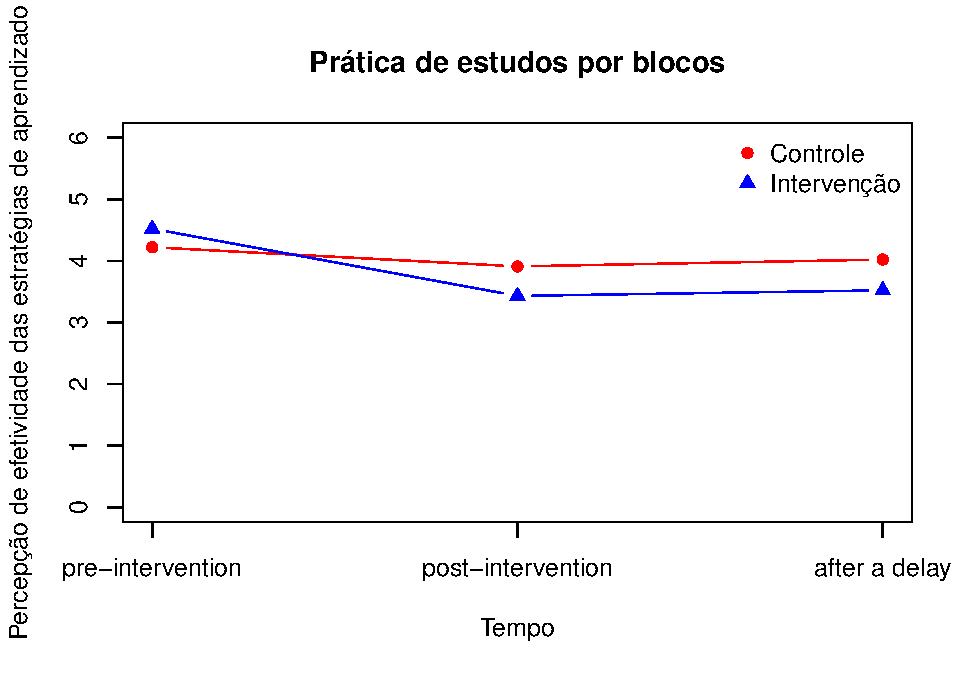
\includegraphics{Projeto_em_grupo_versao-2--pdf-_files/figure-latex/unnamed-chunk-18-1.pdf}
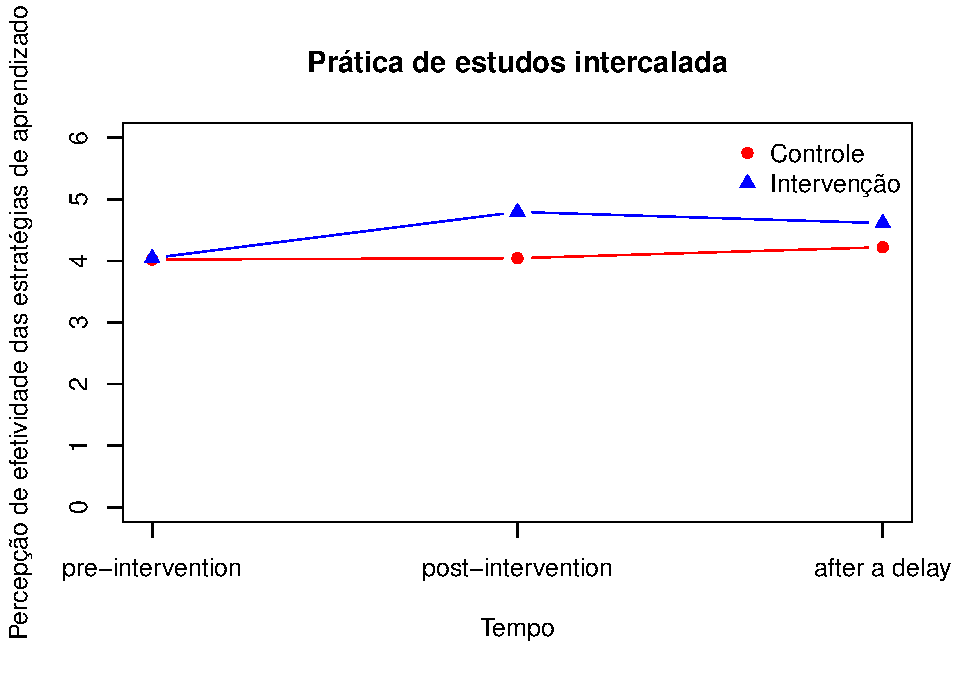
\includegraphics{Projeto_em_grupo_versao-2--pdf-_files/figure-latex/unnamed-chunk-18-2.pdf}

\textbf{RQ3. A prática de estudos intercalada possui algum efeito sobre
a acurácia de classificação?}

\begin{itemize}
\tightlist
\item
  Figura do autor
\end{itemize}

\begin{figure}
\centering
\includegraphics[width=12cm,height=\textheight]{"G:/Meu Drive/UFABC/BC&T/8º quad/Bioestatística/bioestatistica_projeto_final/arquivos_importantes_projeto_dados_imagens/Imagens/grafico_RQ1.png"}
\caption{The use of interleaved practice (in proportions) across
learning tasks}
\end{figure}

\begin{itemize}
\tightlist
\item
  Figura autoral
\end{itemize}

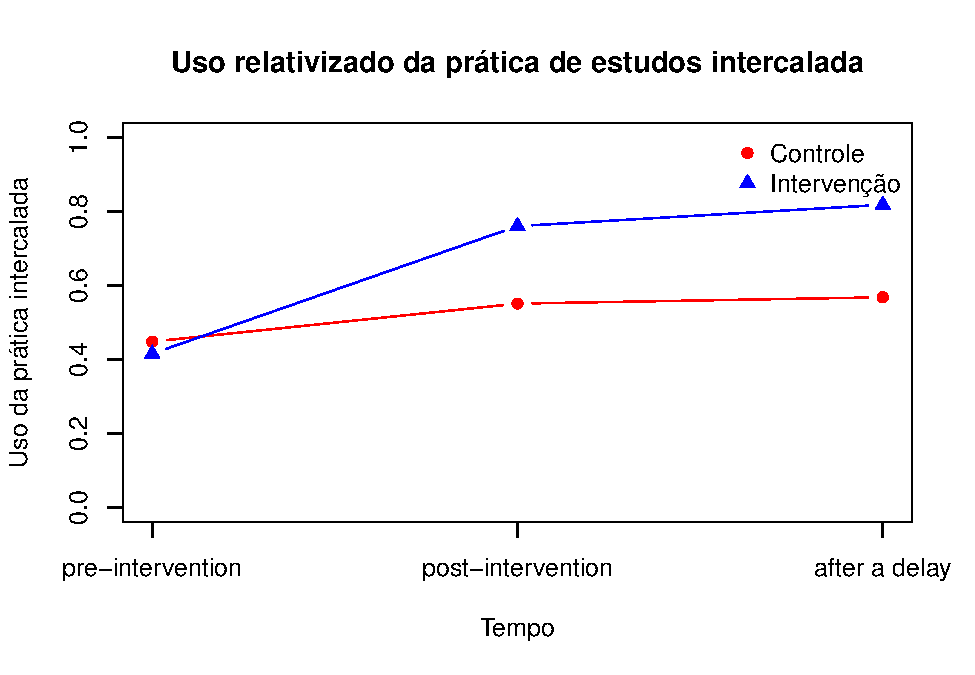
\includegraphics{Projeto_em_grupo_versao-2--pdf-_files/figure-latex/unnamed-chunk-19-1.pdf}

\subsection{Conclusões}\label{conclusuxf5es}

Através dessa pesquisa, é possível visualizar que existem diferentes
formas de estudo, sendo que algumas se apresentam mais eficazes em
detrimento de outras. Os autores apontam que a refutação foi uma
estratégia conveniente do processo, por ter ``forçado'' os estudantes a
questionarem-se e assim, entender de fato um determinado assunto.

Assim, torna-se viável que o método aplicado nessa pesquisa seja
utilizado por universitários (ou estudantes, de um modo geral). É
relevante mencionar que quando existe um interesse particular - ou o
oposto - em uma categoria estudada, o comportamento dos estudantes
frente aos estudos pode apresentar variações. Ademais, os autores
sugerem que pesquisas futuras podem averiguar a eficácia da metodologia
em situações cotidianas.

\end{document}
